Como habíamos mencionado anteriormente, el objetivo del trabajo es encontrar las raíces de $f(x)=x^{2} - \alpha$ y $e(x) = 1/x^{2} - \alpha$.
Para resolver el problema, implementamos para ambas funciones los cuatro métodos iterativos vistos en clase : Bisección, Newton, Regula Falsi y Secante.
La explicación y la base teórica de los mismos puede ser encontrada fácilmente en distintos libros de métodos numéricos, como
por ejemplo: "Numerical Analysis, Burden \& Faires". 

\subsection{Estructura del código}

Antes de comenzar a escribir código decidimos realizar una breve etapa de diseño, en donde nos propusimos encapsular algunos comportamientos para poder escribir un programa
más prolijo y legible.

Lo primero que hicimos fue diseñar una clase llamada $Funciones$. La idea es la siguiente: sea $h$ la función que estamos analizando (podría ser tanto $f$ como $e$).
Como los métodos requieren evaluar $h$ para calcular el valor de la sucesión en los términos siguientes (y algunos $h\_derivada$), sería bueno encapsular estos cálculos
con un comportamiento similar al de una ''caja negra'' (la famosa caja negra). Esto es: en lugar de efectuar la operación en el scope de la función que ejecuta el método,
invocamos a $Funciones.h(x)$ o $Funciones.h\_derivada(x)$, desligándonos de la forma en que estas están implementadas.

Esto es particularmente notorio y beneficioso, por ejemplo, para el código de Newton\_e (i.e: método de Newton para la función $e$. De ahora en más utilizarmos esta notación
para referirnos a los distintos algoritmos):

$\displaystyle e\_deriv = \frac{-2}{x^{3}} \Rightarrow x_{n+1} = x_{n} - \frac{\frac{1}{x_{n}^2}-\alpha}{\frac{-2}{x_{n}^{3}}} \Rightarrow 
x_{n+1} = x_{n} + \frac{(x_{n} - \alpha x_{n}^{3})}{2} $ 

Newton\_e encapsula todos esos cálculos mediante las operaciones:

~

$x_{n+1} = x_{n} - \frac{Funciones.e(x_{n})}{Funciones.e\_deriv(x_{n})}$

~

Luego, por razones muy similares a la anterior, decidimos abstarer el funcionamiento de los criterios de parada, mediante una clase llamada $Criterios$. La decisión de
''cuándo parar'' es independiente al algoritmo que está siendo ejecutado. Además, eventualmente queremos evaluar el comportamiento de un mismo método con distintos 
criterios. Tomemos como ejemplo Bisección. Si hubiéramos implementado esa parte dentro del código del método, entonces habríamos tenido algo de este estilo:

~

\begin{algorithmic}
\Function{Biseccion}{seeds $positivo,negativo$}
	\State \ldots
	\While{$!(max\_iteraciones < i \lor |medio_i < medio_{i-1}| < \epsilon| \lor \frac{|medio_i < medio_{i-1}|}{|medio_{i-1}|} < \epsilon \ldots)}$ 
		\State $\displaystyle medio_{i-1} = medio$
		\State $\displaystyle medio_{i} = \frac{positivo_{i}+negativo_{i}}{2}$
		\State \ldots
	\EndWhile
\EndFunction
\end{algorithmic}

~

Por el contrario, utilizando la clase tenemos:

\begin{algorithmic}
	\While{$!criterios.parar(parameters)$}
		\State \ldots
	\EndWhile
\end{algorithmic}

~

La existencia de class Criterios permite agrupar todo el código que esté relacionado con ellos en un solo bloque, con lo cual ahorramos tener que escribirlos
en cada una de las guardas del while de los distintos algoritmos. Al mismo tiempo resalta el aspecto independiente mencionado más arriba: Los criterios de parada son 
independientes a los métodos que los utilizan.


\subsection{Inicios de la experimentación}

\subsubsection{Primeras experimentaciones. Analizando la convergencia de los métodos}

No surgieron inconvenientes demasiado importantes a la hora de pensar y escribir el código, por lo que procedimos a iniciar la experimentación.
Comenzamos analizando el comportamiento de biseccion\_e y biseccion\_f, ya que asumimos que no tendrían mayores dificultades. Para ello, desarrollamos un método llamado
$semilla\_biseccion\_h$, donde($h = f \ o \ h=e$), que devuelve 2 valores: $pos$ y $neg$ tales que $h(pos)\geq0$ y $h(neg)$ < 0. La ventaja fundamental de bisección
se basa en los reducidos requisitos iniciales que exige para garantizar convergencia (simplemente encontrar 2 semillas tales que al evaluarlas en $h$ difieran en signo).

Luego procedimos a analizar la convergencia de los métodos restantes: Newton, Secante y Regula\_Falsi, para ambas funciones. Para todos ellos las condiciones iniciales que garantizan
convergencia son más restrictivas que las de bisección. Básicamente se reducen a encontrar una buena semilla que pertenezca a un entorno ''cercano'' a la raíz que queremos encontrar.
En esta etapa de la experimentación, agregamos una opción en nuestros métodos que permite recibir por stdin (además de alpha), el valor de la semilla inicial (Newton)/ semillas iniciales (Secante, Regula\_Falsi)
con el que queremos que comiencen. 


\subsubsection{Fijando criterios de parada}

En esta etapa de la experimentación procedimos a encontrar un buen criterio que se adaptara a las condiciones de nuestro problema: encontrar las raíces de $f$ y $e$.
Para ello consideramos que un criterio se adapta a las condiciones cuando hace que el método encuentre una buena aproximación a la raíz
teórica sin necesidad de realizar iteraciones innecesarias. 
Los posibles criterios vistos en clase fueron: Error absoluto y relativo entre iteraciones sucesivas, error absoluto y relativo entre imágenes de iteraciones sucesivas y
valor absoluto de la imagen actual (Ver apéndice: Criterios de parada).
Antes de comenzar las pruebas realizamos una serie de análisis de las funciones y luego planteamos ciertas hipótesis respecto a lo que sucedería.

Supongamos que queremos analizar el comportamiento del siguiente criterio:
$|f(x_{n})| < \epsilon $

¿Es este un buen criterio para encontrar la raíz de f? ¿Podría pasar que el método deje de iterar porque la cota ya ha sido alcanzada pero la solución obtenida esté lejos de la 
raíz teórica?

Sea $f(x) = x^{2} - \alpha$, y dos valores $a, \ b=(a+\delta) \  \in R$ Entonces $|f(a) - f(b)| = |a^{2} - \alpha - ((a+\delta)^{2} - \alpha )| = |a^{2} - \alpha - (a^{2}+\delta^{2}+2*a*\delta) + \alpha | =
|-\delta^{2}-2*a*\delta|$

Podemos deducir el hecho de que:

Si $\delta$ es un valor peque\~no $\Rightarrow \ f(a) \approx f(b) $

Si $\delta$ es un valor grande $\Rightarrow \ f(a) << f(b) $

Por lo tanto, si $|f(x_{n})| < \epsilon \ \Rightarrow |f(x_{n}) - f(\sqrt{\alpha})| < \epsilon \ \Rightarrow x_{n} \approx \sqrt{\alpha}$

~

¿Sucede lo mismo con la función $e$? Sea $e(x) = \frac{1}{x^{2}} - \alpha$ y dos valores $a, \ b=(a+\delta) \in R$. 

Entonces $|e(a) - e(b)| = |\frac{1}{a^{2}} - \alpha - (\frac{1}{(a+\delta)^{2}} - \alpha) | =
|\frac{1}{a^{2}} - \frac{1}{a^{2}+\delta^{2}+2*a*\delta|} | = | \frac{a^{2}+\delta^{2}+2*a*\delta-a^{2}}{a^{2}*(a^{2}+\delta^{2}+2*a*\delta)} | = |\frac{\delta^{2}+2*a*\delta}{a^{4}+a^{2}*\delta^{2}+2*a*\delta}|$

Observemos que el denominador de la última expresión tiene un $a^{4}$ como sumando. Por lo tanto, podría suceder que 2 valores fuesen muy lejanos entre sí ($\delta$ grande), y que sin embargo no exista
tanta diferencia entre sus imágenes. Esto sucede, por ejemplo, cuando $a$ toma valores muy grandes.

En estos casos, podría pasar que $|f(x_{n})| < \epsilon$, y sin embargo $x_{n} >> \frac{1}{\sqrt{\alpha}}$ o $x_{n} << \frac{1}{\sqrt{\alpha}}$

\begin{figure}[!h]
	\begin{center}
		  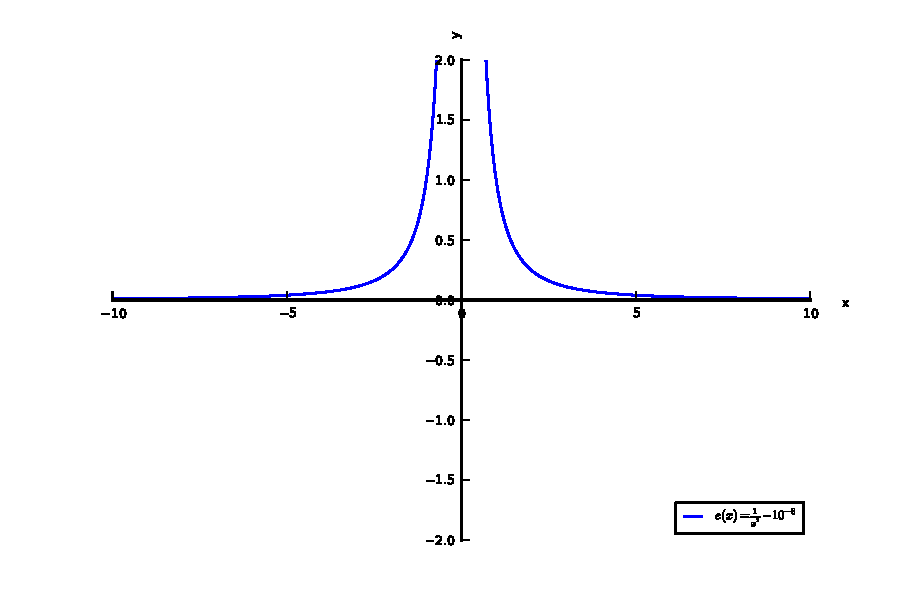
\includegraphics[keepaspectratio]{../Imagenes/exp3/raiz_10000.pdf}
		  \caption{e(x), con $\alpha=10^{-8}$ y $raiz=\frac{1}{\sqrt{\alpha}}=10000$ }
		  \label{fig:contra1}
	\end{center}
\end{figure}
\FloatBarrier

Por ejemplo, para la función $e(x)=\frac{1}{x^2}-10^{-8}$ se cumple que $|e(100)| < 10^{-4}$, y sin embargo el valor de la raíz es $x=10000 >> 100$

Otra de las hipótesis planteadas en esta etapa fue que el criterio 6) $\frac{f(x_{n})-f(x_{n-1})}{f(x_{n-1})}$ funcionaría muy bien, ya que es bastante más estricto que los demás porque incluye en el denominador
un número muy peque\~no.

\subsection{Estableciendo una buena semilla}



